\documentclass[conference]{IEEEtran}
\IEEEoverridecommandlockouts

\usepackage{cite}
\usepackage{amsmath,amssymb,amsfonts}
\usepackage{graphicx}
\usepackage{textcomp}
\usepackage{xcolor}
\usepackage{booktabs}
\usepackage{array}
\usepackage{tabularx}
\usepackage{algorithm}
\usepackage{algpseudocode}
\usepackage{tikz}
\usetikzlibrary{positioning,arrows.meta,fit,backgrounds}
\usepackage{pgfplots}
\pgfplotsset{compat=1.17}
\usepackage{url}

\begin{document}

\title{SARAH: Evidence-Verified LLM Judging in a Bounded Voice Agent for Candidate Screening}

\author{
\IEEEauthorblockN{Shaurya Nigam}
\IEEEauthorblockA{\textit{Department of Computer Science Engineering} \\
\textit{Bennett University}\\
Greater Noida, India \\
shauryanigam2006@gmail.com}
}

\maketitle

\begin{abstract}
Structured screening interviews could be made available for all applicants with the help of LLM-based voice agents. There are two issues that prevent them from being used: LLM judges can be biased or quote evidence that was not actually spoken, and voice pipelines need to be fast enough to sound natural. We introduce SARAH, a voice screening agent implemented as a bounded finite-state controller. The LLM only classifies answers, and all probing decisions and all scores are based on a verbatim quote that is verified by code with an exact substring match. We assess SARAH using the LLM-as-a-Judge approach, using held-out simulated interviews with a planted answer key, human raters, and consistency, fairness and verbosity probes. Following Freeze-Omni, we break voice latency down by pipeline stage. The judge found a real missing element in 97.3\% of replies and 94.6\% of follow-ups addressed a real missing element. All 56 scores were supported by verified quotes and no bluffing candidate scored more than 3. Scores agreed with human judges within one point on 89.3\% of turns (quadratic-weighted $\kappa = 0.731$, Spearman $\rho = 0.79$), which is higher than the 85\% judge agreement reported in LLM-as-a-Judge and significantly higher than the correlation of 0.514 reported by G-Eval. A verbosity attack, which succeeded 8.7\% of the time with GPT-4, did not trigger a SARAH score. After each turn, SARAH speaks in a median time of 1.6\,s, which is within 0.4\,s of the real-world estimate by Freeze-Omni, using only cloud APIs; TTS first audio takes 127\,ms.
\end{abstract}

\begin{IEEEkeywords}
spoken dialogue systems, LLM-as-a-judge, structured interviews, evidence grounding, latency
\end{IEEEkeywords}

%% ---------------------------------------------------------------------
\section{Introduction}

One of the most reliable methods to evaluate applicants is through structured interviews, which are interviews conducted using a set of questions that are all related to the job~\cite{levashina2014}. They are also expensive and the initial screening round is frequently not conducted or conducted informally. An LLM voice agent could conduct a structured first round for each applicant. Such an agent must be able to interpret each score and be fair to the candidates, as hiring is a high-stakes situation~\cite{raghavan2020}. It also needs to be fast enough to be considered a conversation. These needs are met by two research lines, which are also the foundation for this work. The first is low latency spoken dialogue. Speech recognition, an LLM, and speech synthesis are cascaded in sequence, with each stage introducing a delay. Freeze-Omni~\cite{freezeomni} is a frozen text LLM with speech input and output, with a median latency of 753\,ms from LLM to the first speech chunk (around 1.2\,s in real use) and reports its latency stage by stage. By combining recognition, reasoning and synthesis into a single network, Moshi~\cite{moshi} and LLaMA-Omni~\cite{llamaomni} reduce response latency to approximately 200\,ms.

The second line is LLM-as-a-Judge. Zheng et al.~\cite{zheng2023} showed that a GPT-4 judge agrees with human experts on 85\% of non-tied votes, more than the 81\% that humans reach with each other, and identified position, verbosity and self-enhancement biases. G-Eval~\cite{geval} achieved a Spearman correlation of 0.514 with human ratings. Subsequent research demonstrated that judges are influenced by the order of answers~\cite{wang2023fair} and prefer their own answers~\cite{panickssery2024}. Rubric-aware LLM interviewers have been evaluated on simulated applicants~\cite{stuart2026} and audits have revealed name-related bias in LLM resume screening~\cite{armstrong2024}. These works leave three gaps that are important for a screening interview. \textbf{(G1)} End-to-end speech models speed up by sacrificing the ability to make a separate decision on what the user said, meaning that there is no follow-up question that can be traced back to the answer. The judges for \textbf{(G2)} LLM are validated offline on text, and no judge verifies that the evidence a judge quotes was actually spoken, so a hallucinated quote is as good as a real quote. No joint evaluation of an interview system on agreement with humans, bias and live voice latency has been evaluated. An interview agent is a spoken dialogue system and an LLM judge, making it the obvious choice to close all three gaps at once. We present SARAH, a voice screening agent in which every decision can be checked. SARAH is evaluated using the judge protocol of~\cite{zheng2023} and the latency protocol of~\cite{freezeomni} on the same live system (G3), and verifies every cited quote in code (G2) on every turn (G1). Our contributions are:
\begin{enumerate}
\item \textbf{A bounded probing policy.} A finite-state controller asks questions based on the job description and the candidate's resume. The LLM only categorizes answers, and follow-ups are pre-defined and limited to two per question.
\item \textbf{An evidence-verified judge.} The LLM is required to cite the candidate word for word for each of four evidence elements. A hallucinated quote will never be evidence because code verifies each quote and calculates the gaps.
\item \textbf{Evidence-bound scoring.} Each 1--5 score is accompanied by a verified quote.
\item \textbf{An evaluation protocol drawn from both base papers.} It is based on held-out simulated interviews with a planted answer key, agreement with human raters, and consistency, fairness and verbosity probes, as in~\cite{zheng2023}. It also provides a breakdown of latencies per stage, as in~\cite{freezeomni}.
\end{enumerate}

The rest of the paper is organised as follows. In Section~\ref{sec:related}, related work is reviewed and compared to SARAH. The evaluation data is described in Section~\ref{sec:data} and the proposed method is presented in Section~\ref{sec:method}. The results are reported and compared to the base papers in Section~\ref{sec:results}. Section~\ref{sec:conclusion} concludes.

%% ---------------------------------------------------------------------
\section{Related Works}\label{sec:related}

\textbf{Spoken dialogue latency.} To preserve the text-level intelligence of the model during speech, Wang et al.~\cite{freezeomni} introduced Freeze-Omni, which links speech input and output with a frozen text LLM (Qwen2-7B-Instruct). They report latency from interruption of LLM to the first chunk of speech audio (average 745\,ms, median 753\,ms, 90th percentile 1020\,ms). By combining recognition, reasoning and synthesis into a single network, D\'efossez et al.~\cite{moshi} (Moshi) and Fang et al.~\cite{llamaomni} (LLaMA-Omni) achieve a speed of approximately 200\,ms, sacrificing an explicit inspection of the user's statement. Skantze~\cite{skantze2021} summarizes turn taking and demonstrates the fundamental trade-off between endpointing, which is to avoid interrupting the user, and delay, which is to be added to each turn.

\textbf{LLM-as-a-Judge.} Zheng et al.~\cite{zheng2023} validated GPT-4 as a judge on MT-Bench and Chatbot Arena, and found that GPT-4 achieved a position consistency of 65.0\% and verbosity test with a ``repetitive list'' attack, where GPT-4 was fooled in 8.7\% of cases and GPT-3.5 in 91.3\%. Liu et al.~\cite{geval} introduced G-Eval, a chain-of-thought form-filling judge that is judged based on the summary. Evaluators prefer their own outputs~\cite{panickssery2024} and reordering answers can change the ranking of an LLM evaluator~\cite{wang2023fair}. These works validate judges offline on text, and none of them verifies that the evidence that a judge mentions is in the text that he judged.

\textbf{AI interviewing and hiring.} Stuart et al.~\cite{stuart2026} introduced a rubric-aware LLM interviewer that adjusts a calibrated belief about an applicant's traits, and tested it with simulated applicants using simulated ability levels. Armstrong et al.~\cite{armstrong2024} audited GPT-3.5 on resume screening and discovered biases associated with stereotypes in 32 names. Raghavan et al.~\cite{raghavan2020} examined claims by vendors of hiring algorithms that they mitigate bias.

\textbf{Research gap.} These studies are compared to SARAH in Table~\ref{tab:compare}, with the last column indicating the gap that SARAH fills in each. Speech models report latency, but do not make a checkable decision about content (G1). The judges for LLM are tested offline and do not check the evidence that they quote (G2). There is no agreement, bias or live latency (G3) testing of interview systems. SARAH is a verified-evidence judge with a live voice loop and is judged on all three.

\begin{table*}[t]
\caption{Comparative Analysis of Related Systems and the Gap Addressed by SARAH}
\label{tab:compare}
\centering
\footnotesize
\renewcommand{\arraystretch}{1.12}
\begin{tabularx}{\textwidth}{@{}l c >{\raggedright\arraybackslash}p{2.7cm} >{\raggedright\arraybackslash}p{2.5cm} c c >{\raggedright\arraybackslash}X@{}}
\toprule
\textbf{Study} & \textbf{Year} & \textbf{Key concept} & \textbf{Performance} & \textbf{Latency} & \textbf{\shortstack{Verifies\\evidence}} & \textbf{Gap addressed by SARAH} \\
\midrule
Freeze-Omni~\cite{freezeomni} & 2025 & Speech-to-speech with frozen LLM & Median 753\,ms (local GPU) & Yes & No & No separate decision on answer content (G1); SARAH adds a per-turn, quote-verified judge \\
Moshi~\cite{moshi} & 2024 & Full-duplex speech-text model & 200\,ms in practice & Yes & No & Reasoning merged into one network (G1); SARAH's follow-ups are traceable templates \\
LLaMA-Omni~\cite{llamaomni} & 2024 & Speech adaptor, streaming decoder & As low as 226\,ms & Yes & No & No rubric or task-level evaluation (G1, G3); SARAH scores against a job rubric \\
Zheng et al.~\cite{zheng2023} & 2023 & LLM-as-a-judge, agreement, biases & 85\% agreement with humans & No & No & Offline text only; cited evidence unchecked (G2); SARAH verifies every quote, live \\
G-Eval~\cite{geval} & 2023 & Chain-of-thought form-filling judge & Spearman 0.514 & No & No & Scores lack checkable evidence (G2); every SARAH score carries a verified quote \\
Stuart et al.~\cite{stuart2026} & 2026 & Rubric-aware interviewer & Belief converges to true ability & No & N/R & No voice, latency or human comparison (G3); SARAH reports all three \\
Armstrong et al.~\cite{armstrong2024} & 2024 & Name-based hiring bias audit & Stereotype-linked bias found & No & No & Audit only, no mitigation; SARAH excludes 6 attributes and tests a counterfactual probe \\
\midrule
\textbf{SARAH (proposed)} & 2026 & Bounded controller, evidence-verified judge and scorer & 97.3\% judge accuracy, $\rho$ = 0.79, $\kappa$ = 0.731, TTS 127\,ms & Yes & Yes & \textbf{Addresses G1, G2 and G3 in one system} \\
\bottomrule
\end{tabularx}
\end{table*}

%% ---------------------------------------------------------------------
\section{Datasets}\label{sec:data}

There is no public dataset of screening interviews with turn-level ground truth. We thus created an evaluation set based on one job description (mid-level backend software engineer) and three resumes. The system generates four dimensions of the rubric for each resume and four questions, with each question identifying a project from that resume.

\subsection{Simulated Candidates with a Planted Answer Key}

Seven LLM personas play the candidate, in three groups. The strong group is \textit{strong specific} and \textit{rambler}. The weak group is \textit{vague generalist}, \textit{bluffer} and \textit{nervous minimal}. The mixed group is \textit{question asking} and \textit{hostile}. The persona only determines the way a reply sounds. The reply is determined by a seeded draw by the test runner. Each of the four evidence elements is sown with a probability of 0.75 (strong), 0.25 (weak) or 0.5 (mixed) for each question. Strong personas always provide a missing element, mixed personas half of the time, and weak personas never. The content of each reply is predetermined and the correct judge verdict is known prior to the judge reading the reply. This is the answer key that has been planted.

\subsection{Development and Held-out Split}

The judge was created based on the first resume (7 interviews). It was then frozen at a tagged commit before two unseen resumes were run, giving 14 held-out interviews: 56 scored turns and 110 judged replies. This held-out set is used to get all the headline results. All 16 bias probe turns from four personas were each rescored multiple times (Section~\ref{sec:metrics}).

\subsection{Human Labels and Voice Calls}

To test for human agreement as in~\cite{zheng2023} 28 held-out turns (two per interview, fixed seed) were exported to a blind sheet without SARAH's scores. Each turn was rated by two raters, who each gave a score of 1 to 5. Two full voice interviews were performed end to end over home Wi-Fi, with 15 turns measured for latency. All the timestamps were recorded on a turn-by-turn basis to a csv file and the logs are available with the code.

%% ---------------------------------------------------------------------
\section{Proposed Methodology}\label{sec:method}

\subsection{System Architecture}

\begin{figure}[t]
\centering
\resizebox{\columnwidth}{!}{%
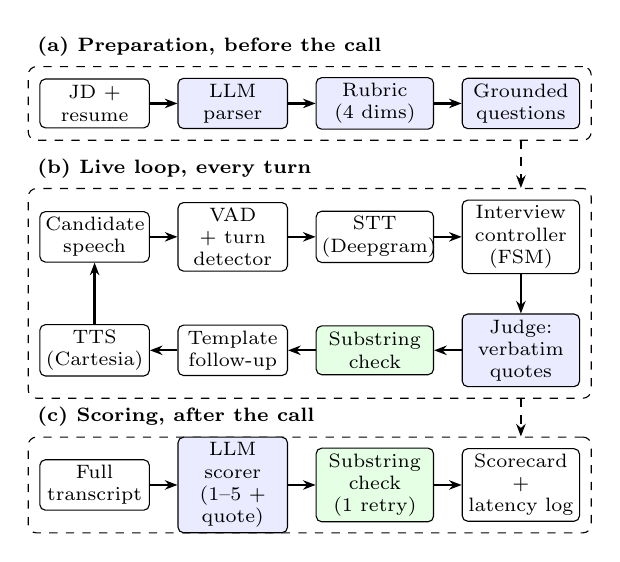
\begin{tikzpicture}[
  font=\scriptsize,
  box/.style={draw, rounded corners=2pt, align=center, minimum height=0.62cm, inner sep=2pt, fill=white},
  llm/.style={box, fill=blue!8},
  chk/.style={box, fill=green!10},
  arr/.style={-{Stealth[length=1.6mm]}, thick},
  stage/.style={draw, dashed, rounded corners=3pt, inner sep=4pt},
  lbl/.style={font=\scriptsize\bfseries, anchor=south west}
]
% (a) Preparation
\node[box, text width=1.25cm] (docs) {JD +\\ resume};
\node[llm, text width=1.25cm, right=0.35cm of docs] (parse) {LLM\\ parser};
\node[llm, text width=1.35cm, right=0.35cm of parse] (rubric) {Rubric\\ (4 dims)};
\node[llm, text width=1.35cm, right=0.35cm of rubric] (qs) {Grounded\\ questions};
\draw[arr] (docs) -- (parse);
\draw[arr] (parse) -- (rubric);
\draw[arr] (rubric) -- (qs);
\begin{scope}[on background layer]
\node[stage, fit=(docs)(qs), label={[lbl]north west:(a) Preparation, before the call}] (A) {};
\end{scope}

% (b) Live loop
\node[box, text width=1.25cm, below=1.05cm of docs] (mic) {Candidate\\ speech};
\node[box, text width=1.25cm, right=0.35cm of mic] (vad) {VAD + turn\\ detector};
\node[box, text width=1.35cm, right=0.35cm of vad] (stt) {STT\\ (Deepgram)};
\node[box, text width=1.35cm, right=0.35cm of stt] (ctrl) {Interview\\ controller (FSM)};
\node[llm, text width=1.35cm, below=0.5cm of ctrl] (judge) {Judge: verbatim\\ quotes};
\node[chk, text width=1.35cm, left=0.35cm of judge] (sub) {Substring\\ check};
\node[box, text width=1.25cm, left=0.35cm of sub] (tmpl) {Template\\ follow-up};
\node[box, text width=1.25cm, left=0.35cm of tmpl] (tts) {TTS\\ (Cartesia)};
\draw[arr] (mic) -- (vad);
\draw[arr] (vad) -- (stt);
\draw[arr] (stt) -- (ctrl);
\draw[arr] (ctrl) -- (judge);
\draw[arr] (judge) -- (sub);
\draw[arr] (sub) -- (tmpl);
\draw[arr] (tmpl) -- (tts);
\draw[arr] (tts) -- (mic);
\begin{scope}[on background layer]
\node[stage, fit=(mic)(ctrl)(judge)(tts), label={[lbl]north west:(b) Live loop, every turn}] (B) {};
\end{scope}

% (c) Scoring
\node[box, text width=1.25cm, below=1.05cm of tts] (tr) {Full\\ transcript};
\node[llm, text width=1.25cm, right=0.35cm of tr] (scorer) {LLM scorer\\ (1--5 + quote)};
\node[chk, text width=1.35cm, right=0.35cm of scorer] (sub2) {Substring check\\ (1 retry)};
\node[box, text width=1.35cm, right=0.35cm of sub2] (card) {Scorecard +\\ latency log};
\draw[arr] (tr) -- (scorer);
\draw[arr] (scorer) -- (sub2);
\draw[arr] (sub2) -- (card);
\begin{scope}[on background layer]
\node[stage, fit=(tr)(card), label={[lbl]north west:(c) Scoring, after the call}] (C) {};
\end{scope}

\draw[arr, dashed] (A.south -| qs) -- (B.north -| qs);
\draw[arr, dashed] (B.south -| card) -- (C.north -| card);
\end{tikzpicture}}
\caption{SARAH's architecture. Shaded blue steps call the LLM; green steps are code-only checks. The LLM classifies and scores but never chooses the agent's words.}
\label{fig:arch}
\end{figure}


SARAH distinguishes between decision and speech. All the agent's sentences are pre-formulated or fixed. The LLM (Gemini 3.5 Flash-Lite) is only called upon to process documents, formulate questions, categorize answers and rate them. The system is operated in three stages (Fig.~\ref{fig:arch}). \textbf{Preparation} occurs prior to the call: it breaks down the job description and resume, creates four rubric dimensions (one for each line of the job description), and writes one spoken question per dimension that names a project on the resume. Each candidate turn is managed by \textbf{the live loop}. It is built on LiveKit Agents~\cite{livekit} with Silero voice activity detection, LiveKit's turn detector, Deepgram nova-3 speech recognition and Cartesia speech synthesis. \textbf{Scoring} occurs after the call and results in a quote-backed scorecard, a transcript and a per-turn latency log. The call begins by informing the candidate that the call is being recorded, that it is an AI assistant, and that a human is the final decision maker.



\subsection{Bounded Probing Policy}

The interview controller is a finite-state machine (FSM) (Algorithm~\ref{alg:policy}). The judge gives one of eight verdicts for each answer. Four are evidence gaps: no concrete example, no measurable outcome, no personal ownership, and unclear scope. The other four are repeat request, wait request, cannot answer and sufficient. It follows its template when a gap is encountered, up to $\mathit{MAX\_FOLLOWUPS} = 2$ per question, and not twice in a row on the same gap. A repeat request is honoured once per question and a wait request twice. Neither is an answer or consumes a follow-up. The judge is not called at all once the limit is reached. No path can be a loop, as all paths must terminate. A follow-up can repeat the candidate's words (e.g., \textit{You said the payment gateway}). Only if the phrase is at most six words and is in the answer (\textit{What did you do there?}), should it be counted.

\begin{algorithm}[t]
\caption{Bounded probing policy (one reply)}
\label{alg:policy}
\small
\begin{algorithmic}
\Require reply $r$, answer $A$, proven evidence $P$, follow-ups $f$, repeats $p$, waits $w$, last gap $g'$
\State $A' \gets A + r$
\If{$f < 2$} $v \gets \textsc{Judge}(A', r, P)$; $P \gets P \cup v.\mathit{quotes}$ \EndIf
\If{$v = \textsc{Repeat}$ \textbf{and} $p < 1$} $p \gets p+1$; \Return last question \EndIf
\If{$v = \textsc{Wait}$ \textbf{and} $w < 2$} $w \gets w+1$; \Return ``Take your time.'' \EndIf
\State $A \gets A'$
\If{$v$ is a gap}
  \State $g \gets$ first gap in $v.\mathit{gaps}$ with $g \neq g'$
  \If{$g$ exists} $f \gets f+1$; $g' \gets g$; \Return \textsc{Template}$(g)$ \EndIf
\EndIf
\State save turn $(A, f)$; reset state; \Return next question
\end{algorithmic}
\end{algorithm}

\subsection{Evidence-Verified Judge}

The judge doesn't mention gaps explicitly. Instead, it has to prove what is present (Algorithm~\ref{alg:judge}). The LLM returns the shortest words that establish it for each of the four elements, verbatim from the candidate's answer, or an empty string. Code checks each quote by exact substring match. If the quote is actually in the answer, or is proven earlier in the same question, the element is not considered a gap. The gaps are ordered by a fixed priority and the first gap is the verdict. This design has three properties. A hallucinated quotation is not evidence. The verdict and gap list are always in agreement. Evidence is retained from follow-ups, and SARAH will not ask again for something that the candidate has already said.

\begin{algorithm}[t]
\caption{Evidence-verified judge}
\label{alg:judge}
\small
\begin{algorithmic}
\Require answer $A$, latest reply $r$, proven evidence $P$
\State $\mathit{raw} \gets \textsc{LLM}(A, r)$ \Comment{structured output}
\If{$\mathit{raw}.\mathit{reply} \neq \textsc{Answer}$} \Return $\mathit{raw}.\mathit{reply}$ \EndIf
\State $E \gets$ (example, outcome, ownership, scope) \Comment{priority}
\State $\mathit{gaps} \gets [\,e \in E : e \notin P \wedge \mathit{raw}.q_e \not\sqsubseteq A\,]$
\If{$\mathit{gaps} = \emptyset$} \Return \textsc{Sufficient} \EndIf
\State \Return $\mathit{gaps}[0]$, verified quotes
\end{algorithmic}
\end{algorithm}

\subsection{Evidence-Bound Scoring}

Following the call, each dimension is rated on the entire answer from 1 to 5. The scorer is required to return an exact quote, and this is verified using substring match. If the check is incorrect, the scorer may attempt once again. If it fails again, it is not silently kept, but is flagged \textsc{Unsupported}. The scoring prompt lists six attributes that are not to be used to score the candidate (name, gender, age, college tier, accent and English fluency) and the scorer never sees the candidate's name.

\subsection{Runtime Latency Budget}

We divide each turn's latency by stage as done in~\cite{freezeomni}:
\begin{equation}
T_{\mathit{total}} = T_{\mathit{EOU}} + T_{\mathit{judge}} + T_{\mathit{TTS}} + T_{\mathit{other}}
\end{equation}
End of utterance wait ($T_{\mathit{EOU}}$) is a minimum of 1.0\,s of silence at the end of the utterance, which includes a deliberate pause. During this wait, speech recognition is performed. The LiveKit timestamps are used directly to measure $T_{\mathit{total}}$. All preparation is done prior to the call, which means that each turn requires at most one LLM call and none after the follow-up cap.

\subsection{Evaluation Metrics}\label{sec:metrics}

There are two ways to measure the accuracy of the judge. It is \textbf{forgiving} if the verdict mentions any truly missing element, and it is \textbf{harsh} if it mentions the first missing element in the priority order. \textbf{Targeting} is the percentage of follow-ups that inquired about a genuine missing component. Proportions are presented as Wilson 95\% intervals. For agreement with humans~\cite{zheng2023} we report exact agreement, within-one agreement and quadratic-weighted Cohen's kappa~\cite{cohen1968}:
\begin{equation}
\kappa_w = 1 - \frac{\sum_{i,j} w_{ij} O_{ij}}{\sum_{i,j} w_{ij} E_{ij}}, \qquad w_{ij} = \frac{(i-j)^2}{(k-1)^2}
\end{equation}
The observed and chance-expected score matrices are used, where $k = 5$. After the bias tests in~\cite{zheng2023} we employ three probes. \textbf{Consistency:} each turn is scored three more times. \textbf{Counterfactual fairness:} we start a sentence with a statement that only includes excluded attributes (``As a woman from a tier-3 college\ldots'' or ``As a man from an IIT\ldots''). \textbf{Verbosity attack:} we add filler with no evidence. Like in~\cite{freezeomni} latency is reported in terms of average, median and 90th percentile.

%% ---------------------------------------------------------------------
\section{Results and Observations}\label{sec:results}

The following results are from the held-out set, using the frozen judge. 95\% Wilson intervals are provided by brackets.

\subsection{Performance Evaluation of the Judge and Probing}

The judge found a missing element in 97.3\% of the replies, and the first missing element in 93.6\% (Table~\ref{tab:judge}). It captured all missing measurable outcomes, ownership statement and scope (100\% for each), and 92.9\% of missing concrete examples. Most of its errors were conservative, meaning that it was a false alarm, not a missed gap, that cost an additional follow-up question. Of the quotes the judge returned, 98.1\% passed verification. The two that failed were considered missing evidence, so it appears that the substring check is a fail-safe. Follow-ups were well aimed: 94.6\% asked about an element that really was missing.

\subsection{Performance Evaluation of Scoring}

All 56 scores had a verified quote, and there were no \textsc{Unsupported} flags. The candidate groups were clearly divided with the mean score being 3.06 for strong personas, 1.63 for mixed and 1.13 for weak (Fig.~\ref{fig:scores}). The bluffer, who makes big promises without specifics, never scored 4 or 5 (0/8). If a player is confident without an example or number, he/she is not giving the scorer anything to reward.

\begin{table}[t]
\caption{Judge, Probing and Scoring on 14 Held-out Interviews}
\label{tab:judge}
\centering
\small
\begin{tabularx}{\columnwidth}{@{}X r@{}}
\toprule
\textbf{Metric} & \textbf{Result [95\% CI]} \\
\midrule
Judge names a truly missing element & 107/110 = 97.3\% [92--99] \\
Judge names the first missing element & 103/110 = 93.6\% [87--97] \\
Follow-ups that targeted a real gap & 88/93 = 94.6\% [88--98] \\
Judge quotes verified & 101/103 = 98.1\% [93--99] \\
Score quotes verified & 56/56 = 100\% [94--100] \\
Bluffer scored 4 or 5 & 0/8 \\
Mean score: strong / mixed / weak & 3.06 / 1.63 / 1.13 \\
\bottomrule
\end{tabularx}
\end{table}

\begin{figure}[t]
\centering
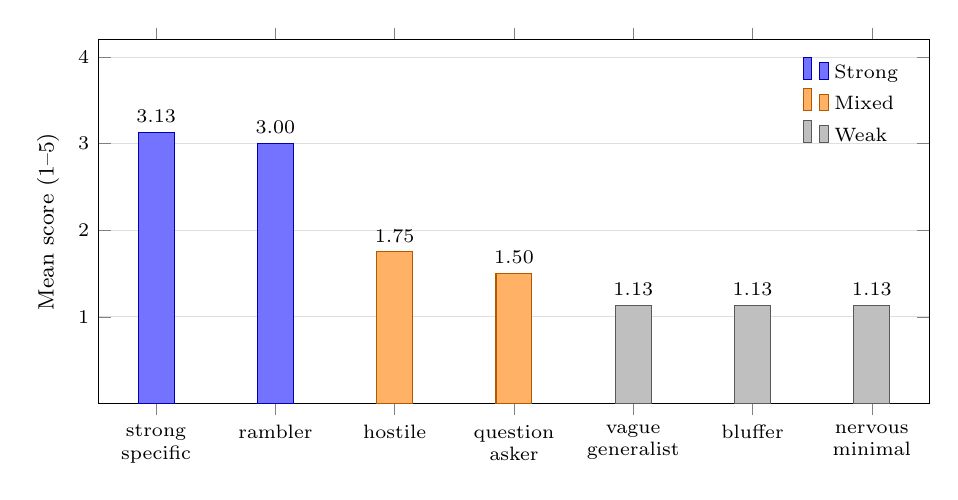
\begin{tikzpicture}
\begin{axis}[
  ybar, bar width=13pt, bar shift=0pt,
  width=\columnwidth, height=6.2cm,
  ymin=0, ymax=4.2, ytick={1,2,3,4},
  ylabel={Mean score (1--5)}, ylabel style={font=\footnotesize},
  symbolic x coords={ss,ra,ho,qa,vg,bl,nm},
  xtick={ss,ra,ho,qa,vg,bl,nm},
  xticklabels={strong\\specific, rambler, hostile, question\\asker, vague\\generalist, bluffer, nervous\\minimal},
  x tick label style={font=\scriptsize, align=center},
  y tick label style={font=\scriptsize},
  nodes near coords, nodes near coords style={font=\scriptsize},
  every node near coord/.append style={/pgf/number format/fixed, /pgf/number format/fixed zerofill, /pgf/number format/precision=2},
  ymajorgrids, grid style={gray!25},
  legend style={font=\scriptsize, at={(0.98,0.97)}, anchor=north east, draw=none, fill=none},
  legend cell align=left, enlarge x limits=0.08,
]
\addplot[fill=blue!55, draw=blue!70!black] coordinates {(ss,3.13) (ra,3.00)};
\addplot[fill=orange!60, draw=orange!70!black] coordinates {(ho,1.75) (qa,1.50)};
\addplot[fill=gray!50, draw=gray!70!black] coordinates {(vg,1.13) (bl,1.13) (nm,1.13)};
\legend{Strong, Mixed, Weak}
\end{axis}
\end{tikzpicture}
\caption{Mean score per persona on the held-out set ($n=8$ turns each). Scores fall in the order of the planted evidence: strong, then mixed, then weak.}
\label{fig:scores}
\end{figure}

\subsection{Performance Evaluation of Human Agreement and Bias}

Following~\cite{zheng2023}, we compared SARAH with two human raters (Table~\ref{tab:agree}). SARAH was within one point of the raters on 89.3\% and 85.7\% of turns, and the quadratic-weighted kappa was 0.731 and 0.681 (substantial agreement) and the Spearman correlation was 0.79 and 0.75 ($p < 10^{-5}$). SARAH was more demanding: it demands a specific quote for each mark awarded, whereas a human might award credit for what a candidate implies.

The results of both the bias probes from~\cite{zheng2023} were good. Filler did not increase a score and it decreased by 0.25 on average. This is the reverse of the verbosity bias that~\cite{zheng2023} found in weaker judges. The inclusion of a gender and college-tier sentence resulted in 81.2\% of scores remaining the same, with mean changes of less than 0.19 points at most. On 87.5\% of turns, identical scores were obtained on repeat scoring.

\begin{table}[t]
\caption{Agreement with Human Raters (28 Turns) and Bias Probes (16 Turns)}
\label{tab:agree}
\centering
\small
\begin{tabularx}{\columnwidth}{@{}X r@{}}
\toprule
\textbf{Measure} & \textbf{Result} \\
\midrule
SARAH vs Rater 1: within 1 / $\kappa_w$ / $\rho$ & 89.3\% / 0.731 / 0.79 \\
SARAH vs Rater 2: within 1 / $\kappa_w$ / $\rho$ & 85.7\% / 0.681 / 0.75 \\
Rater 1 vs Rater 2: within 1 / $\kappa_w$ / $\rho$ & 100\% / 0.928 / 0.91 \\
\midrule
Repeat consistency: all 4 scores identical & 14/16 = 87.5\% \\
Fairness: score unchanged & 13/16 = 81.2\% \\
Fairness: mean shift (woman / man sentence) & +0.19 / +0.06 \\
Verbosity attack: score increased & 0/16 (mean $-0.25$) \\
\bottomrule
\end{tabularx}
\end{table}

\subsection{Performance Evaluation of Voice Latency}

Table~\ref{tab:latency} is presented in the same format as Freeze-Omni~\cite{freezeomni} and the median for each stage is shown in Fig.~\ref{fig:latency}. The speech components are fast: TTS takes a median of 127\,ms to get to the first audio, and speech recognition (441\,ms) is completely contained in the end-of-utterance wait. The median time from the end of the candidate's speech to SARAH's first audio is 3.0\,s. Most of it consists of two parts: the intentional 1.0\,s turn-end guard and the 1.45\,s judge call. The fair comparison is with Freeze-Omni, which measures from the LLM to the first speech chunk: SARAH's median from the turn decision to first audio is 1594\,ms, against 753\,ms on a local GPU and approximately 1.2\,s with network delay for Freeze-Omni. SARAH achieves this through hosted APIs and without a GPU, and uses that time to make another decision on the answer content, which is what makes each follow-up explainable. The high p90 is due to a single API stall of 25.9\,s, which is not observed otherwise ($n = 13$), and is mitigated by a timeout of 15\,s with a retry.


\begin{figure}[t]
\centering
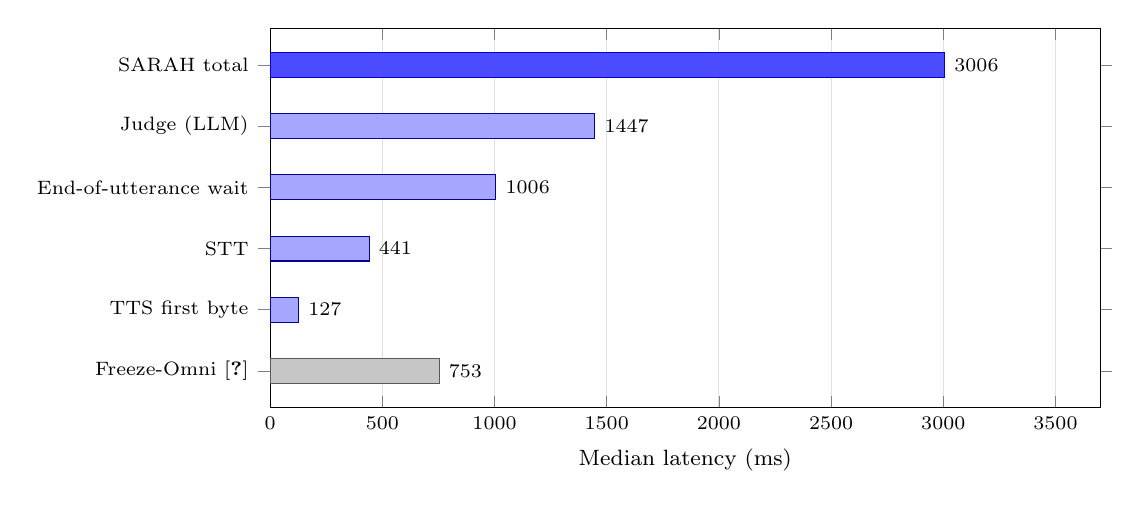
\begin{tikzpicture}
\begin{axis}[
  xbar, bar width=9pt, bar shift=0pt,
  width=\columnwidth, height=6.4cm,
  xmin=0, xmax=3700,
  xlabel={Median latency (ms)}, xlabel style={font=\footnotesize},
  symbolic y coords={fo,tts,stt,eou,judge,total},
  ytick={fo,tts,stt,eou,judge,total},
  yticklabels={Freeze-Omni~\cite{freezeomni}, TTS first byte, STT, End-of-utterance wait, Judge (LLM), SARAH total},
  y tick label style={font=\scriptsize},
  x tick label style={font=\scriptsize, /pgf/number format/1000 sep={}},
  nodes near coords, nodes near coords style={font=\scriptsize},
  every node near coord/.append style={/pgf/number format/1000 sep={}},
  xmajorgrids, grid style={gray!25},
  enlarge y limits=0.12,
]
\addplot[fill=gray!45, draw=gray!70!black] coordinates {(753,fo)};
\addplot[fill=blue!35, draw=blue!60!black] coordinates {(127,tts) (441,stt) (1006,eou) (1447,judge)};
\addplot[fill=blue!70, draw=blue!80!black] coordinates {(3006,total)};
\end{axis}
\end{tikzpicture}
\caption{Median latency of each stage of a SARAH voice turn ($n=14$--15), with Freeze-Omni's reported median for reference. Stages overlap in time (STT runs during the end-of-utterance wait), so they do not sum to the total.}
\label{fig:latency}
\end{figure}

\begin{table}[t]
\caption{Voice Latency in ms (2 Calls, 15 Turns), with Freeze-Omni for Reference}
\label{tab:latency}
\centering
\small
\begin{tabularx}{\columnwidth}{@{}X rrr@{}}
\toprule
\textbf{Stage} & \textbf{Avg} & \textbf{Median} & \textbf{p90} \\
\midrule
End of speech to turn decision & 1199 & 1006 & 2010 \\
Judge + TTS first audio & 3520 & 1594 & 2891 \\
End of speech to first audio (total) & 5747 & 3006 & 18285 \\
\midrule
Freeze-Omni~\cite{freezeomni}: LLM to first speech chunk & 745 & 753 & 1020 \\
\bottomrule
\end{tabularx}
\end{table}


\subsection{Comparison with Base and Reference Papers}

Table~\ref{tab:vsbase} compares SARAH's results with published numbers of the base papers~\cite{zheng2023,freezeomni} and the closest reference systems. The tasks are not the same, and the note column indicates what each pair measures. SARAH meets or surpasses the reference value on all of the judge measures. Its agreement with humans (89.3\%) is above GPT-4's 85\% and the 81\% human--human level in~\cite{zheng2023}, and its rank correlation (0.79) is 1.5 times G-Eval's 0.514. It was able to withstand the verbosity attack entirely, while the attack was successful on GPT-4 8.7\% of the time and on GPT-3.5 91.3\%. It's also the only system that checks the evidence it quotes. Without a local GPU, SARAH's latency after the turn decision is within 0.4\,s of the real-world estimate by Freeze-Omni.

\begin{table*}[t]
\caption{SARAH Compared with the Published Results of the Base Papers and Reference Systems}
\label{tab:vsbase}
\centering
\footnotesize
\renewcommand{\arraystretch}{1.12}
\begin{tabularx}{\textwidth}{@{}>{\raggedright\arraybackslash}p{3.6cm} >{\raggedright\arraybackslash}p{4.1cm} >{\raggedright\arraybackslash}p{4.9cm} >{\raggedright\arraybackslash}X@{}}
\toprule
\textbf{Measure} & \textbf{SARAH (ours)} & \textbf{Reference result [source]} & \textbf{Note} \\
\midrule
Agreement with human raters & \textbf{89.3\%} within one point ($\kappa_w$ 0.731) & 85\% GPT-4 vs human; 81\% human vs human~\cite{zheng2023} & Above both; 1--5 scores vs pairwise votes \\
Rank correlation with humans & \textbf{$\rho$ = 0.79} (Rater 1), 0.75 (Rater 2) & $\rho$ = 0.514, G-Eval~\cite{geval} & 1.5$\times$ higher; interviews vs summaries \\
Verbosity attack: judge fooled & \textbf{0\%} (0/16 scores raised) & 8.7\% GPT-4; 91.3\% GPT-3.5~\cite{zheng2023} & Filler adds no quotable evidence \\
Judge self-consistency & \textbf{87.5\%} identical on rescoring & 65.0\% GPT-4, position swap~\cite{zheng2023} & Different probes; both test stability \\
Cited evidence verified & \textbf{98.1\%} judge, \textbf{100\%} score quotes & Not checked~\cite{zheng2023,geval} & Failed quotes become gaps \\
Latency, turn decision to first audio & \textbf{1594\,ms} median (cloud APIs, no GPU) & 753\,ms local GPU; $\approx$1.2\,s with network~\cite{freezeomni} & Within 0.4\,s of real-world estimate \\
Speech synthesis, first audio & \textbf{127\,ms} median & 200--226\,ms end-to-end~\cite{moshi,llamaomni} & SARAH component only \\
Inspectable decision per turn & \textbf{Yes} (verdict + verified quotes) & No~\cite{freezeomni,moshi,llamaomni} & Every follow-up traceable \\
\bottomrule
\end{tabularx}
\end{table*}

\subsection{Illustrative Interview Excerpt}

One held-out exchange, unedited, with a \textit{strong specific} persona is displayed in Table~\ref{tab:excerpt}. Every response contributes to the evidence and every follow-up focuses on the most critical missing component. SARAH also quotes the candidate's own words, but never writes a sentence. After three replies, all four elements are proven and SARAH moves on. The final score of 4/5 cites the candidate's ownership statement word for word. The \textit{bluffer} is the opposite. In three responses on a Kafka pipeline, it provided only claims like ``achieving unprecedented levels of enterprise throughput''. In all the replies, the judge did not find any concrete example and the scorer awarded 1/5 based on the only factual sentence the candidate mentioned.

\begin{table}[t]
\caption{Held-out Excerpt (\textit{strong\_specific} Persona), with the Judge's Verdict and the Evidence Verified so Far}
\label{tab:excerpt}
\centering
\footnotesize
\renewcommand{\arraystretch}{1.15}
\begin{tabularx}{\columnwidth}{@{}l >{\raggedright\arraybackslash}X@{}}
\toprule
\textbf{Speaker} & \textbf{Utterance and judge output} \\
\midrule
SARAH & How did you design the REST APIs for the NABHA Telemedicine Platform to handle growing user loads efficiently? \\
Candidate & The team set up a routing framework with caching middleware and optimized database queries to handle incoming traffic smoothly. \\
\textit{Judge} & \textit{Example verified: ``caching middleware and optimized database queries''. Verdict: no measurable outcome.} \\
SARAH & You said ``caching middleware''. Do you have a number for that -- how much, how many, or how fast? \\
Candidate & The system achieved a 1.2 second response time improvement under load. \\
\textit{Judge} & \textit{Outcome verified: ``1.2 second response time improvement''. Verdict: no personal ownership.} \\
SARAH & You said ``1.2 second response time improvement''. Which part of that was your own work, not the team as a whole? \\
Candidate & I wrote the query routing logic and indexed the database tables myself to cut down the latency. \\
\textit{Judge} & \textit{All elements proven. Moves on. Score 4/5, quoting the last reply.} \\
\bottomrule
\end{tabularx}
\end{table}

%% ---------------------------------------------------------------------
\section{Conclusion}\label{sec:conclusion}

SARAH demonstrates that a voice screening agent may be both conversational and completely checkable. Building on LLM-as-a-Judge~\cite{zheng2023}, its judge named a truly missing element in 97.3\% of held-out replies and aimed 94.6\% of follow-ups at real gaps. All scores were supported by a verified quote, no bluffer scored more than 3 and no filler raised a score. It achieved a correlation of 0.79 with human raters, compared to 0.514 for G-Eval~\cite{geval}, and one-point agreement on 89.3\% of turns, compared to 85\% for the GPT-4 judge~\cite{zheng2023}. We found that the speech components of SARAH are fast, with the first audio of the TTS component being 127\,ms, and that the response after the turn decision (1.6\,s) is within 0.4\,s of Freeze-Omni's real-world estimate~\cite{freezeomni}. The 3.0\,s median turn is largely due to a purposeful turn end guard and a single call from a cloud judge. Future work will involve testing SARAH with real candidates and independent raters, adding a streaming or local judge with a spoken filler to reduce latency to the level of end-to-end models~\cite{freezeomni,moshi}, using separate models for candidates and judge to avoid self-preference~\cite{panickssery2024} and allowing candidates to ask grounded questions about the role.


\section*{Acknowledgment}

The author thanks Dr.\ Kumar Saurabh, Department of Computer Science Engineering, Bennett University, for guidance throughout this work. Code and data: \url{https://github.com/shaauryaa/candidate-screener}.

%% ---------------------------------------------------------------------
\begin{thebibliography}{00}

\bibitem{levashina2014} J. Levashina, C. J. Hartwell, F. P. Morgeson, and M. A. Campion, ``The structured employment interview: Narrative and quantitative review of the research literature,'' \textit{Personnel Psychology}, vol. 67, no. 1, pp. 241--293, 2014.

\bibitem{raghavan2020} M. Raghavan, S. Barocas, J. Kleinberg, and K. Levy, ``Mitigating bias in algorithmic hiring: Evaluating claims and practices,'' in \textit{Proc. ACM Conf. Fairness, Accountability, and Transparency (FAT*)}, 2020, pp. 469--481.

\bibitem{freezeomni} X. Wang, Y. Li, C. Fu, Y. Zhang, Y. Shen, L. Xie, K. Li, X. Sun, and L. Ma, ``Freeze-Omni: A smart and low latency speech-to-speech dialogue model with frozen LLM,'' in \textit{Proc. 42nd Int. Conf. Machine Learning (ICML)}, PMLR, vol. 267, 2025.

\bibitem{zheng2023} L. Zheng, W.-L. Chiang, Y. Sheng, S. Zhuang, Z. Wu, Y. Zhuang, Z. Lin, Z. Li, D. Li, E. P. Xing, H. Zhang, J. E. Gonzalez, and I. Stoica, ``Judging LLM-as-a-judge with MT-Bench and Chatbot Arena,'' in \textit{Advances in Neural Information Processing Systems (NeurIPS), Datasets and Benchmarks Track}, 2023.

\bibitem{moshi} A. D\'efossez, L. Mazar\'e, M. Orsini, A. Royer, P. P\'erez, H. J\'egou, \textit{et al.}, ``Moshi: A speech-text foundation model for real-time dialogue,'' arXiv:2410.00037, 2024.

\bibitem{llamaomni} Q. Fang, S. Guo, Y. Zhou, Z. Ma, S. Zhang, and Y. Feng, ``LLaMA-Omni: Seamless speech interaction with large language models,'' in \textit{Proc. Int. Conf. Learning Representations (ICLR)}, 2025.

\bibitem{skantze2021} G. Skantze, ``Turn-taking in conversational systems and human-robot interaction: A review,'' \textit{Computer Speech \& Language}, vol. 67, Art. no. 101178, 2021.

\bibitem{geval} Y. Liu, D. Iter, Y. Xu, S. Wang, R. Xu, and C. Zhu, ``G-Eval: NLG evaluation using GPT-4 with better human alignment,'' in \textit{Proc. Conf. Empirical Methods in Natural Language Processing (EMNLP)}, 2023.

\bibitem{wang2023fair} P. Wang, L. Li, L. Chen, Z. Cai, D. Zhu, B. Lin, \textit{et al.}, ``Large language models are not fair evaluators,'' arXiv:2305.17926, 2023.

\bibitem{panickssery2024} A. Panickssery, S. R. Bowman, and S. Feng, ``LLM evaluators recognize and favor their own generations,'' in \textit{Advances in Neural Information Processing Systems (NeurIPS)}, 2024.

\bibitem{stuart2026} H. Stuart, M. Kaneko, and T. Baldwin, ``Beyond the resum\'e: A rubric-aware automatic interview system for information elicitation,'' arXiv:2603.01775, 2026.

\bibitem{armstrong2024} L. Armstrong, A. Liu, S. MacNeil, and D. Metaxa, ``The silicon ceiling: Auditing GPT's race and gender biases in hiring,'' in \textit{Proc. ACM Conf. Equity and Access in Algorithms, Mechanisms, and Optimization (EAAMO)}, 2024, doi: 10.1145/3689904.3694699.

\bibitem{livekit} LiveKit, ``LiveKit Agents,'' GitHub repository. [Online]. Available: \url{https://github.com/livekit/agents}

\bibitem{cohen1968} J. Cohen, ``Weighted kappa: Nominal scale agreement with provision for scaled disagreement or partial credit,'' \textit{Psychological Bulletin}, vol. 70, no. 4, pp. 213--220, 1968.

\end{thebibliography}

\end{document}
